% Chapter Template

\chapter{Model} % Main chapter title

\label{Chapter4} % Change X to a consecutive number; for referencing this chapter elsewhere, use \ref{ChapterX}

%----------------------------------------------------------------------------------------

% Define some commands to keep the formatting separated from the content 
\newcommand{\keyword}[1]{\textbf{#1}}
\newcommand{\tabhead}[1]{\textbf{#1}}
\newcommand{\code}[1]{\texttt{#1}}
\newcommand{\file}[1]{\texttt{\bfseries#1}}
\newcommand{\option}[1]{\texttt{\itshape#1}}

%----------------------------------------------------------------------------------------

%----------------------------------------------------------------------------------------
%	SECTION 1
%----------------------------------------------------------------------------------------

\section{Introduction}


The problem of generation of a set of chords from a melody is very similar to that of translating one language to another. 
The translation problem is one that is very popular in machine learning research and thus there is many resources on it.  
However the music related problem is harder to solve due to the extra dimension each of its elements contains. 
Each element in a melody has both pitch, represented by a descrete symbol or note, and duration whereas each element in the sequence of language is composed of only the discrete symbols or words.  
Therefore in order to use techniques developed for natural language processing it is necessary to encode the melody and chords in such a way that their dimensions are collapsed into one. 
Since this collapsing of dimensions has already been conducted in \textbf{REF TO DATA CHAPTER} we are able to take full advanatges of NLP techniques.
There has been many attempts to apply some of these techniques to the chord generation problem. 
In order to find the best model we evaluate these attempts against a defined criteria and develop a novel model to evalutate against the same criteria.


\section{Model Requirements}
\subsection{MVP Requrements}

The MVP requirements were defined at the beginning of the project to ensure it is compatible with the other parts of the product that were simaltaniously in development and to ensure the possibbility of the creation of the prototye for proof of concept. 
We required the model to be a black box in which we could input a melody and it would output chords which sounded good.
The notion of sounding good is intentionally vague as what sounds good or bad is usually down to individual taste in music.
There is never a definitive answer to which chords would sound the best.
However, we felt \textbf{NEED STRONGER PROOF} that even people without any musical training would be able to judge whether chords fit the melody relatively accurately.
Within this overarching requirement we defined tighter constraints for the sake of both practicality and user experience. 
The model would have to be designed for sequential data such that the temporal relationship of the different notes being played were taken into account.
It would be possible to simply learn a function where for a given measure a chord suited to the notes played within that measure was generated without taking into account surrounding measures.
This approach could produce reasonable results and be significantly more simple that other options, however, the quality and variation of chords generated would be lower than that of a model for sequential data, hence our choice to forego it.
The model would also have to be conditional. For a given input it should produce a catered output. This is an obious contraint however for models such as a GAN it recquires changes to the format of the input data.
To maximise user experience the models should be non-deterministic. This allows users to regenerate the accompaniment multiple times to obtain new chords and thus means they can choose what they feel is best.
For practicality sake we constrained our MVP to only require one chord to be played each measure as the problem of determining when a chord should be played is of similar difficulty to choosing which chord to play.
\subsection{Other possible Requrements}

There were some constraints which were not used in our project which would provide better quality chords but provided too large a practical barrier to be implemented.
The act of collapsing the pitch and duration of the notes into a single dimension removes information from the melody.
In our case this information is the order in which the notes are played and the rhythmic intention of the composer.
It is likely a model would be able to produce more suitable chords given this information.
Thus, for a stricter set of constrains we could include the requirement that the order and duration of notes are both maintained in the data.
The accompaniment for music is not limited to a single chord played at the start of each bar.
A much more interesting accompaniment would be generated if it were not limited to this restrictive format.
As shown in \cite{ReinforcementLearning} it is possible to create a model which learns the divisons within the music and thus learns when would be most appropriate to play a chord.
Therfore, in order to allow for more interesting accompaniment, the requirement of one chord per bar could be changed such that chords should be played with closer freedom to that of a human composer.
% Strongly temporal

\subsection{Evaluation criteria}
\paragraph{Approach}
Many attempts to solve the chord generation problem have been made each of which containing variants on models and implementations which result in large variations in mertrics used for evaluation.
There is also a large variation in features for which quantative evaluation is impossible. 
As it would be impractical to implement each relevent model ourselves to allow for full standardistation of evaluation we will evaluate models built ourselves and from previous work based on a set of criteria defined below.
\paragraph{Data}
One of the biggest influences on the effectiveness of a model is the dataset on which it is trained. 
In general a larger dataset results in a better generalisation of learning \textbf{Need proof}.
Most datasets are comprised of lead sheets which can be translated into chord melody pairs.
Many datasets are then further divided down into measures in which there is one chord played per measure and the melody within that measure is somehow encoded.
Thus for best comparison the number of measures used in the dataset is a good criterion for evaluation.
This is a particularly important area for evaluation as it will strongly affect the output of the model and thus the results of other 

\paragraph{Quantiative Evalutaion}
There is difficulty in quantative evaluation for this problem as there is no strictly correct chords for a given melody and thus comparison to any specific set of chords gives a skewed interpretation of the output.
However, the use of conventional quantative evaluation does still correlate strongly with the sentiment given by a human judging the quality of chords and thus can be cautionsly used in evalution.
The test set from the data can be used to compare the outputs from the model to previously assigned chords. Accuracy can be found by finding the number of chords successfully predicted and dividing by the total number of chords produced.
\begin{equation}
    \text{Accuracy} = \frac{\text{Number of Chords Correctly Assigned}}{\text{Total Number of Chords Generated}}
\end{equation}
As this was the only quantative measure consistently used across previous implementations this is the only one we will consider for evaluation.

\paragraph{Qualitative Evaluation}
Some previous work \cite{MySong}, \cite{BLSTM} carried out experiments to judge the sentiment of untrained musicicans to the generated chords.
Participants were played the melody accompanied by a varying set of chords and asked to judge which chords they felt were best out of a set containing chords generated by models and some human written accompaniment.
The results from these experiements can be used to compare models to each other as well as evlauate them relative to the standard set by human written chords.
As well as evaluation based on the quality of chords produced we will discuss extra functionality made possible by some models and the effect this has on other evaluation metrics.

\paragraph{Criteria}
The final criteria used for evaluation are thus:
\begin{itemize}
    \item Number of measures in the dataset
    \item Accuracy in testing
    \item Human sentiment towards generated chords
    \item Extra functionality the model provides
\end{itemize}
\section{Models}

The generation of chords to accompany a monphonic melody is an area which has developed as machine learning techniques are improved. 
An early approach to this problem from \cite{ChordPrediction} used a standard MLP to learn the relationship between melodies and accompanying chords.
MySong, the first attempt focusing specifically on a vocal melody in \cite{MySong} used an augment hidden markov model with parameters such that users could adjust the "Happy factor" and "Jazz factor" to alter the mood of the generated chords to their preference.
A weakness of the hidden markov model is that at each timestep only the previous timestep is considers when suggesting a chord. 
\cite{BLSTM} utilises a BLSTM to increase the effect of long term dependencies on the output rather than relying only on the previous output.
\cite{MLForChords} tested and evaluated a number of more simple models such a Logistic Regression, Naive Bayes, SVM and Random Forest trained on data from 43 lead sheets \\
\cite{ReinforcementLearning} proposed a model  that learns a structured representation for use in symbolic melody harmonization. It utilises two layers of LSTMs to detemine when each chord should be played then utilise a policy gradient RL method to select each chord.
MuseGAN \\      
ChordGAN \\       
CLSTMGAN for melody Generation \\

\subsection{Model evaluation template}
Model explanation/history - why is it generally applicable \\
Previous implementaitions \\
    General backgorund \\
    Evaluation \\
        Data \\
        Quantative \\
        Qualitative \\
        Extra features \\
\subsection{HMMs}
\label{subsec:HMM}
\subsubsection{Explanation and Applicability}
Hidden Markov Models or HMMs were first put forward by Leonard E. Baum in a series of statistical papers \textbf{list papers from wikipedia}. 
They model a stochasitc process in which the desired states, $\boldsymbol{X}$, are not directly observable but related states, $\boldsymbol{Y}$, which directly influence the desired states are. 
By modeling the $\boldsymbol{X}$ and $\boldsymbol{Y}$ Markov Processes \textbf{references?} we are able to infer the hidden state.
To apply an HMM to our problem we take the hidden state, $\boldsymbol{X}$, to be the chords played, and the observable state $\boldsymbol{Y}$ to be the Melody.
It is notable that the conditional probability distribution of the hidden variable $x(t)$ at time t, only depends on that of the previous time step $x(t-1)$ and that $y(t)$ only depends on the hidden distribution at the current time step $x(t)$.
For our puroses this limits the "memory" the model could have to a single measure and thus seriously reduces the effect of relationship between chords across time.

\subsubsection{Implementations}

\paragraph{MySong} The first application of an HMM to this problem while also being the the first attempt focusing specifically on a vocal melody from \cite{MySong} used an augmented hidden markov model with parameters such that users could adjust the "Happy factor" and "Jazz factor" to alter the mood of the generated chords to their preference.
No measure was given for the accuracy of the model, however a study which compared the quality of MySong to Manually assigned chords was carried out. 
In 264 comparisons the participants prefered MySon 95 times, manual 121 times and had no preference 48 times
The additional user input possible with the "Happy factor" and "Jazz factor" parameters are reported to significantly improve the user experience, however, this is thier only implementation and so nothing can be infered about the quality of the HMM itself.

\paragraph{Chord Generation from Symbolic Melody}  As a comparison for the main model in \cite{BLSTM} an HMM was implemented. 
The HMM is trained on a reduced version of the \textbf{Include link?} wikifonia.org dataset which includes and array of Western music genres with 2,252 lead sheets, 1802 of which are used for training. 
This overall comes to 72,418 measures for the training set and 17,768 for the test set. 
They tested the accuracy of the HMM on sequences of length 4, 8, 12, and 16 bars long gaining an accuracy of $0.4033$, $0.4043$, $0.4041$, and $0.4045$ respectively and an average accuracy of $0.4041$.
They also carried out a user subjective test with 25 participants each evaluating 18 sets, each set containing a melody acompanied by three generated chord sequences and an original chord sequence.
The users would listen to the music played and judge the accompaniment on a scale of 1, being not appropriate, and 5, being very appropriate.
The HMM achieved an average score of $2.31$ and the original chords achieved an average score of $4.04$.

\paragraph{Machine Learning in Automatic Music Chords Generation} An HMM was tested in \cite{MLForChords} along with other simpler models. It was trained on 43 lead sheets, with 813 measures total. 
An accuracy of $0.4844$ was achieved, however an choice of only 7 chords were used unlike the usual 24.

% \paragraph{Autoarrangement System of Accompaniment Chords} An HMM with improved PCP feature extraction was used in \cite{HMMswithML} 

\subsection{DNN-HMMs}

\label{subsec:DNN-HMMs}
\subsubsection{Explanation and Applicability} 

A deep neural network HMM makes it possible to assume a posterior for the HMM using the output from the softmax output layer of the DNN. 
This allows for the posterior to be learned in training.

\subsubsection{Implementations}

\paragraph{Chord Generation from Symbolic Melody} This was implemented much like the HMM from \cite{BLSTM} mentioned above in \ref{subsec:HMM}.
The same dataset was used and an accuracy of $0.4502$, $0.4482$, $0.4495$, and $0.4468$  was obtained on the 4, 8, 12 and 16 bars respectively. This results in an average accuracy of $0.4487$.
On the user subjective test the DNN-HMM achieved a score of $2.48$.

\subsection{GANs}

\subsubsection{Explanation and Applicability}

Generative Adversarial Netwoks or GANs were first proposed in the landmark paper \cite{GANs}. Unlike most models GANs consist of two separate agents working against each other.
The first model, the Generator, takes an input of random noise and outputs data which mimics the training data. 
The second model, the Discriminator, takes as input an example from the training data or an output from the Generator and outputs a value between 0 and 1 indicating whether it thinks the input is real or generated.
The Binary Cross Entropy loss is used for the Discriminator avaraged across real and generate examples. The loss for the Generator is the log complement of that for the Discriminator. Thus the two models play the following minmax game:
\begin{equation}
\underset{D}{\text{min}} \underset{G}{\text{max}} V(D,G) = \mathbf{E}_{x\sim p_{data}(\mathbf{x})}[logD(\mathbf{x})] + \mathbf{E}_{z\sim p_{data}(\mathbf{z})}[log(1-D(G(\mathbf{z})))]
\end{equation} 
Theoretically the Generator and Discriminator can be any differentaible function thus leaving much room for flexibility.
The problem with GANs for our uses is that they are not conditional, the only input to the Generator is noise. A proposed remody for this was presented in \cite{CGANs}.
By concatinating the label data, in our case the melody, with the noise as input to the Generator and doing the same with the training data and the label data, in our case a chord and melody, as input to the Discriminator GANs can be made conditional. 
Thus they would be suitable for our uses. 

\subsubsection{Implementations}

\paragraph{ChordGAN} \cite{ChordGAN} uses a conditional GAN along with Chroma Feature Extraction to generate chords for a specific genre of music based on the dataset it was trained on.
They used three different data sets one for each Pop, Jazz and Classical music each shorter than 1600 measures (specific lengths are not given).
The model achieved an acuracy of $0.68$, $0.74$ and $0.64$ respectively across the datasets.

\subsection{RNNs}

Recurrent Neural Networks or RNNs have become a staple in the machine learning engineer's library of models. 
They are structured much like a normal MLP, however, they contain an extra connection to the state of the network in the timestep before.
This means that the state of the network at each timestep depends that of the previous timestep and thus the state at the current timestep is affected by the state in all previous timesteps.
This makes RNNs ideal for processing sequential data as temporal relationships are taken into account.
The gradient of RNNs can be found using a variation of the backpropagation algorithm usually know as backpropagation through time.
RNNs that operate on large sequences often experience the probblems of exploding or vanishing gradients leading to a saturation of learning.

\begin{figure}
    \centering
    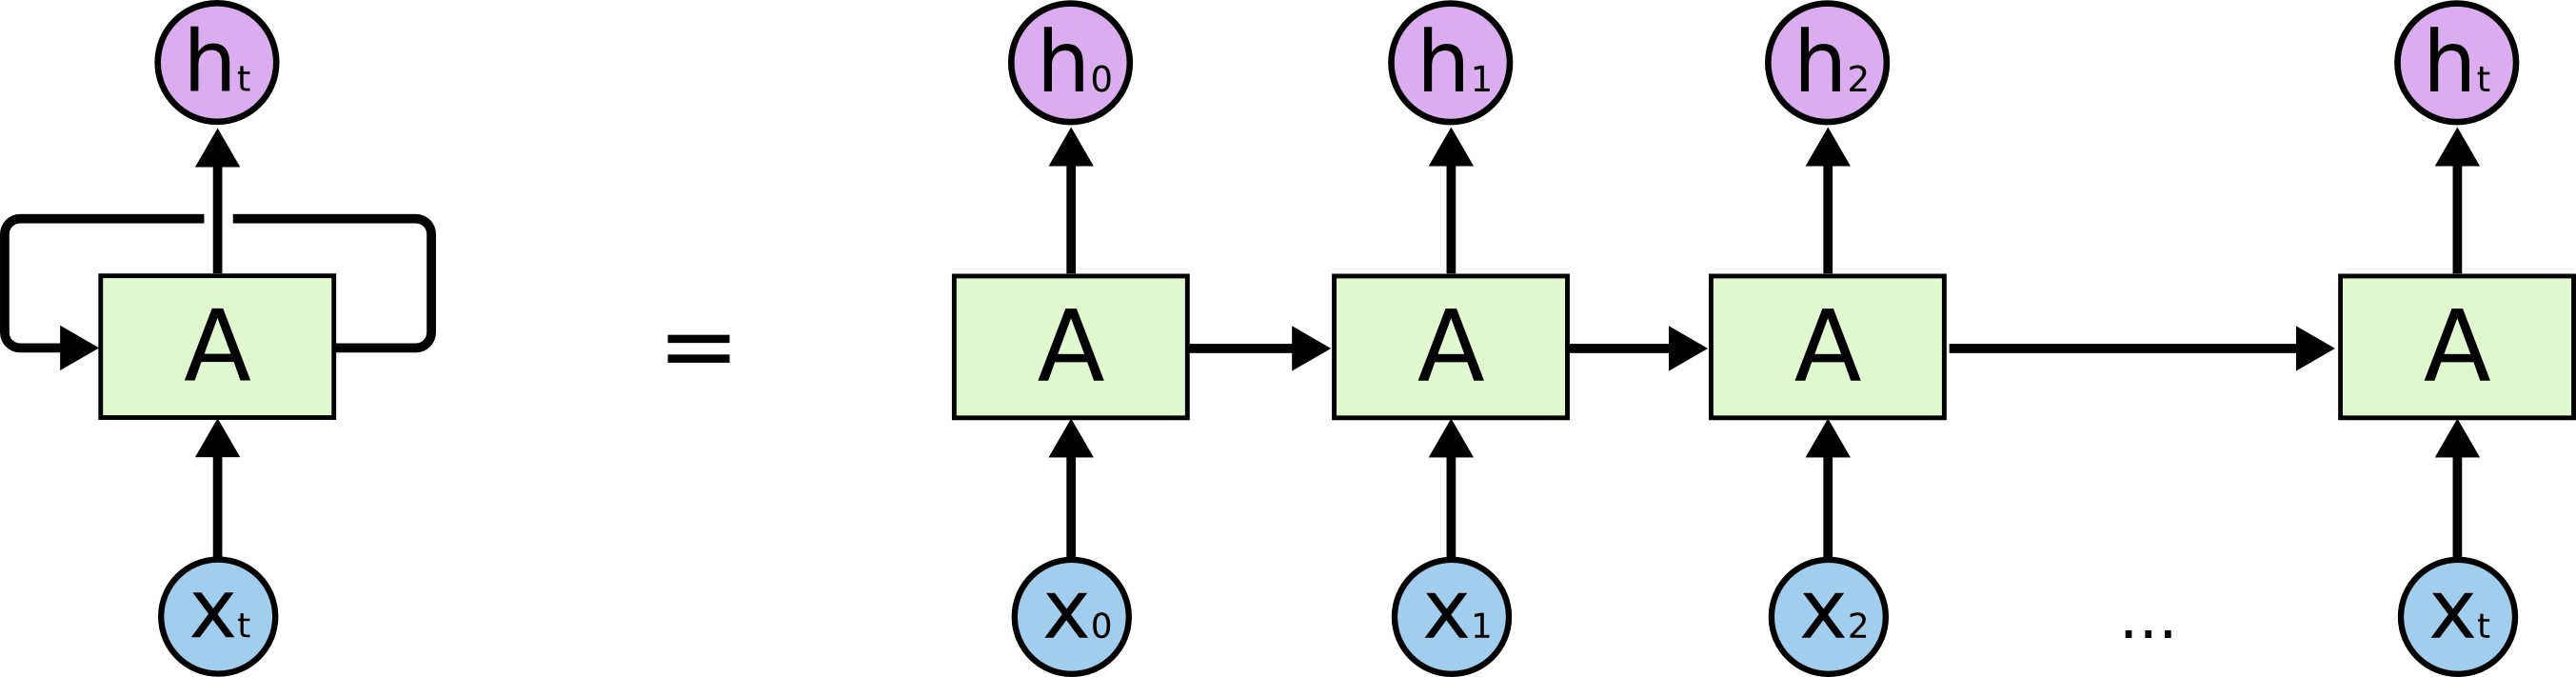
\includegraphics[width=0.8\columnwidth]{Figures/RNN}
    \decoRule
    \caption[An RNN]{A many inputs to many outputs diagram of an RNN from \cite{oinkina}}
    \label{fig:RNN}
\end{figure}

\subsection{LSTMs}

The Long Short Term Memory model or LSTM was proposed in \cite{LSTMs} in order to overcome the gradient problems related to RNNs and thus allow for faster training on long sequences.
They are also capable or learning longer dependencies due to their internal memory. An LSTM cell has three gates: input, forget, and output.
The state of these gates determines whether the cell allows new input, forgets old information, and affects the output at the current timestep.
At timeset t, the states of the gates are given by:
\begin{equation}
    i_t=\sigma(w_i[h_{t-1},x_t]+b_i)
\end{equation}
\begin{equation}
    f_t=\sigma(w_f[h_{t-1},x_t]+b_f)
\end{equation}
\begin{equation}
    o_t=\sigma(w_o[h_{t-1},x_t]+b_o)
\end{equation}
where $i_t$, $f_t$ and $o_t$ denote the input, forget, and output gates state respectively, $h_{t-1}$ is the output at the previous timestep.
$w$ and $b$ represent weights and biases of each gate, $x_t$ is the input to the LSTM cell, and $\sigma (.)$ is the sigmoid function applied elementwise.
The current output of the cell is computed by:
\begin{equation}
    h_t=o_t \circ tanh(c_t)
\end{equation}
\begin{equation}
    c_t = f_t \circ c_{t-1}+i_t \circ \overset{\sim}{c}_t
\end{equation}
\begin{equation}
    \overset{\sim}{c}_t = tanh(w_c[h_t,x_t]+b_c)
\end{equation}

\begin{figure}
    \centering
    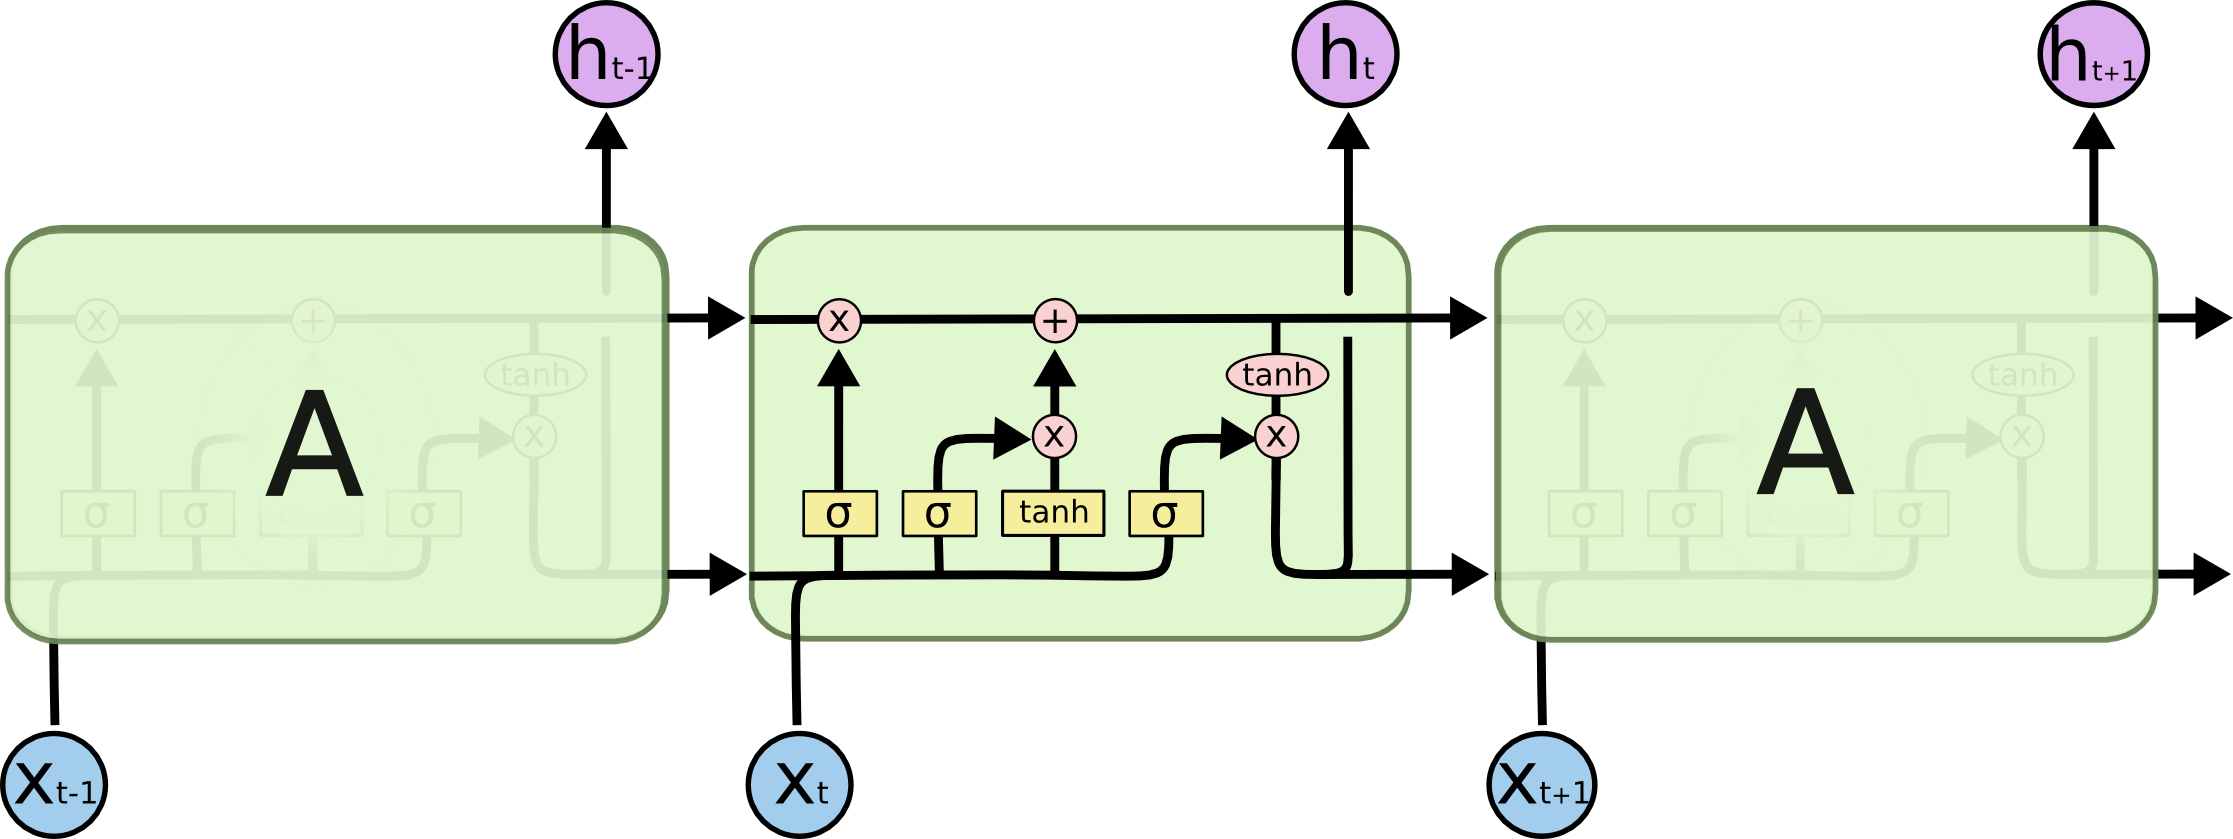
\includegraphics[width=0.8\columnwidth]{Figures/LSTM}
    \decoRule
    \caption{The repeating module in an LSTM from \cite{oinkina}}
    \label{fig:LSTM}
\end{figure}

\subsubsection{Implementations}

\paragraph{Chord Generation from Symbolic Melody} This was the main model under scrutiny in \cite{BLSTM} mentioned above in \ref{subsec:HMM} and \ref{subsec:DNN-HMMs}.
They build a bidirection LSTM with two hidden layers and used a hyperbolic tangent activation function. The softmax function is applied to the output in order to represent the probaility that each of the 24 chords is played.
The same dataset as the HMM and DNN-HMM was used and an accuracy of $0.5055$, $0.5032$, $0.4923$, and $0.4990$  was obtained on the 4, 8, 12 and 16 bars respectively. This results in an average accuracy of $0.5000$.
On the user subjective test the DNN-HMM achieved a score of $3.55$.

\paragraph{Automatic Melody Harmonization} A particularly interesting model heaviliy relying on LSTMs surrounded by a reinforcement learning framework was proposed in \cite{ReinforcementLearning}.
The simultaniously trained a Structured Representation Module responsible for learning note-level, phrase-level and segment level representaitions, a Segmentation Module acting as a reinforcement learning agent to decide whether the current note is the boundary of a phrase or segment and a Harmonisation Module responsible for generating chords for each segment.
They used the Hooktheory Lead Sheet Dataset with 10,000 songs, no number of measures is given but with the differnece in model architecture so drastic a comparison on this metric would be inappropriate anyway.
The achieved an accuracy of $0.3742$ and compared that to an SVM, CNN, LSTM and BLSTM with blocked Gibbs sampling which achieved an accuracy of $0.2516$, $0.2664$, $0.2802$, $0.2933$ respectively.
% The inclusion of variable numbers of chords in each measure greatly expands the possibilities with music composition

\subsection{Transformers}

Transformers have been a revolutionary development in the field of NLP, first proposed by \cite{Transformers} they have become very widely used and regularly produce state of the art performance.
Transformers utilise the encoder decoder model for sequence to sequence translation.
They also heavily use attention which is a mechanism for weighting the importance of different elements of a sequence of data.
Specifically they propose the Scaled dot-product attention shown in \ref{eq:Attention}
\begin{equation}
    \text{Attention}(Q,K,V) = \text{softmax}(\frac{QK^T}{\sqrt{d_k}})V
    \label{eq:Attention}
\end{equation}
where $Q$, $K$ and $V$ represent the queries, keys and values respectively and $d_k$ is the dimension or queries and keys.
\begin{figure}
    \centering
    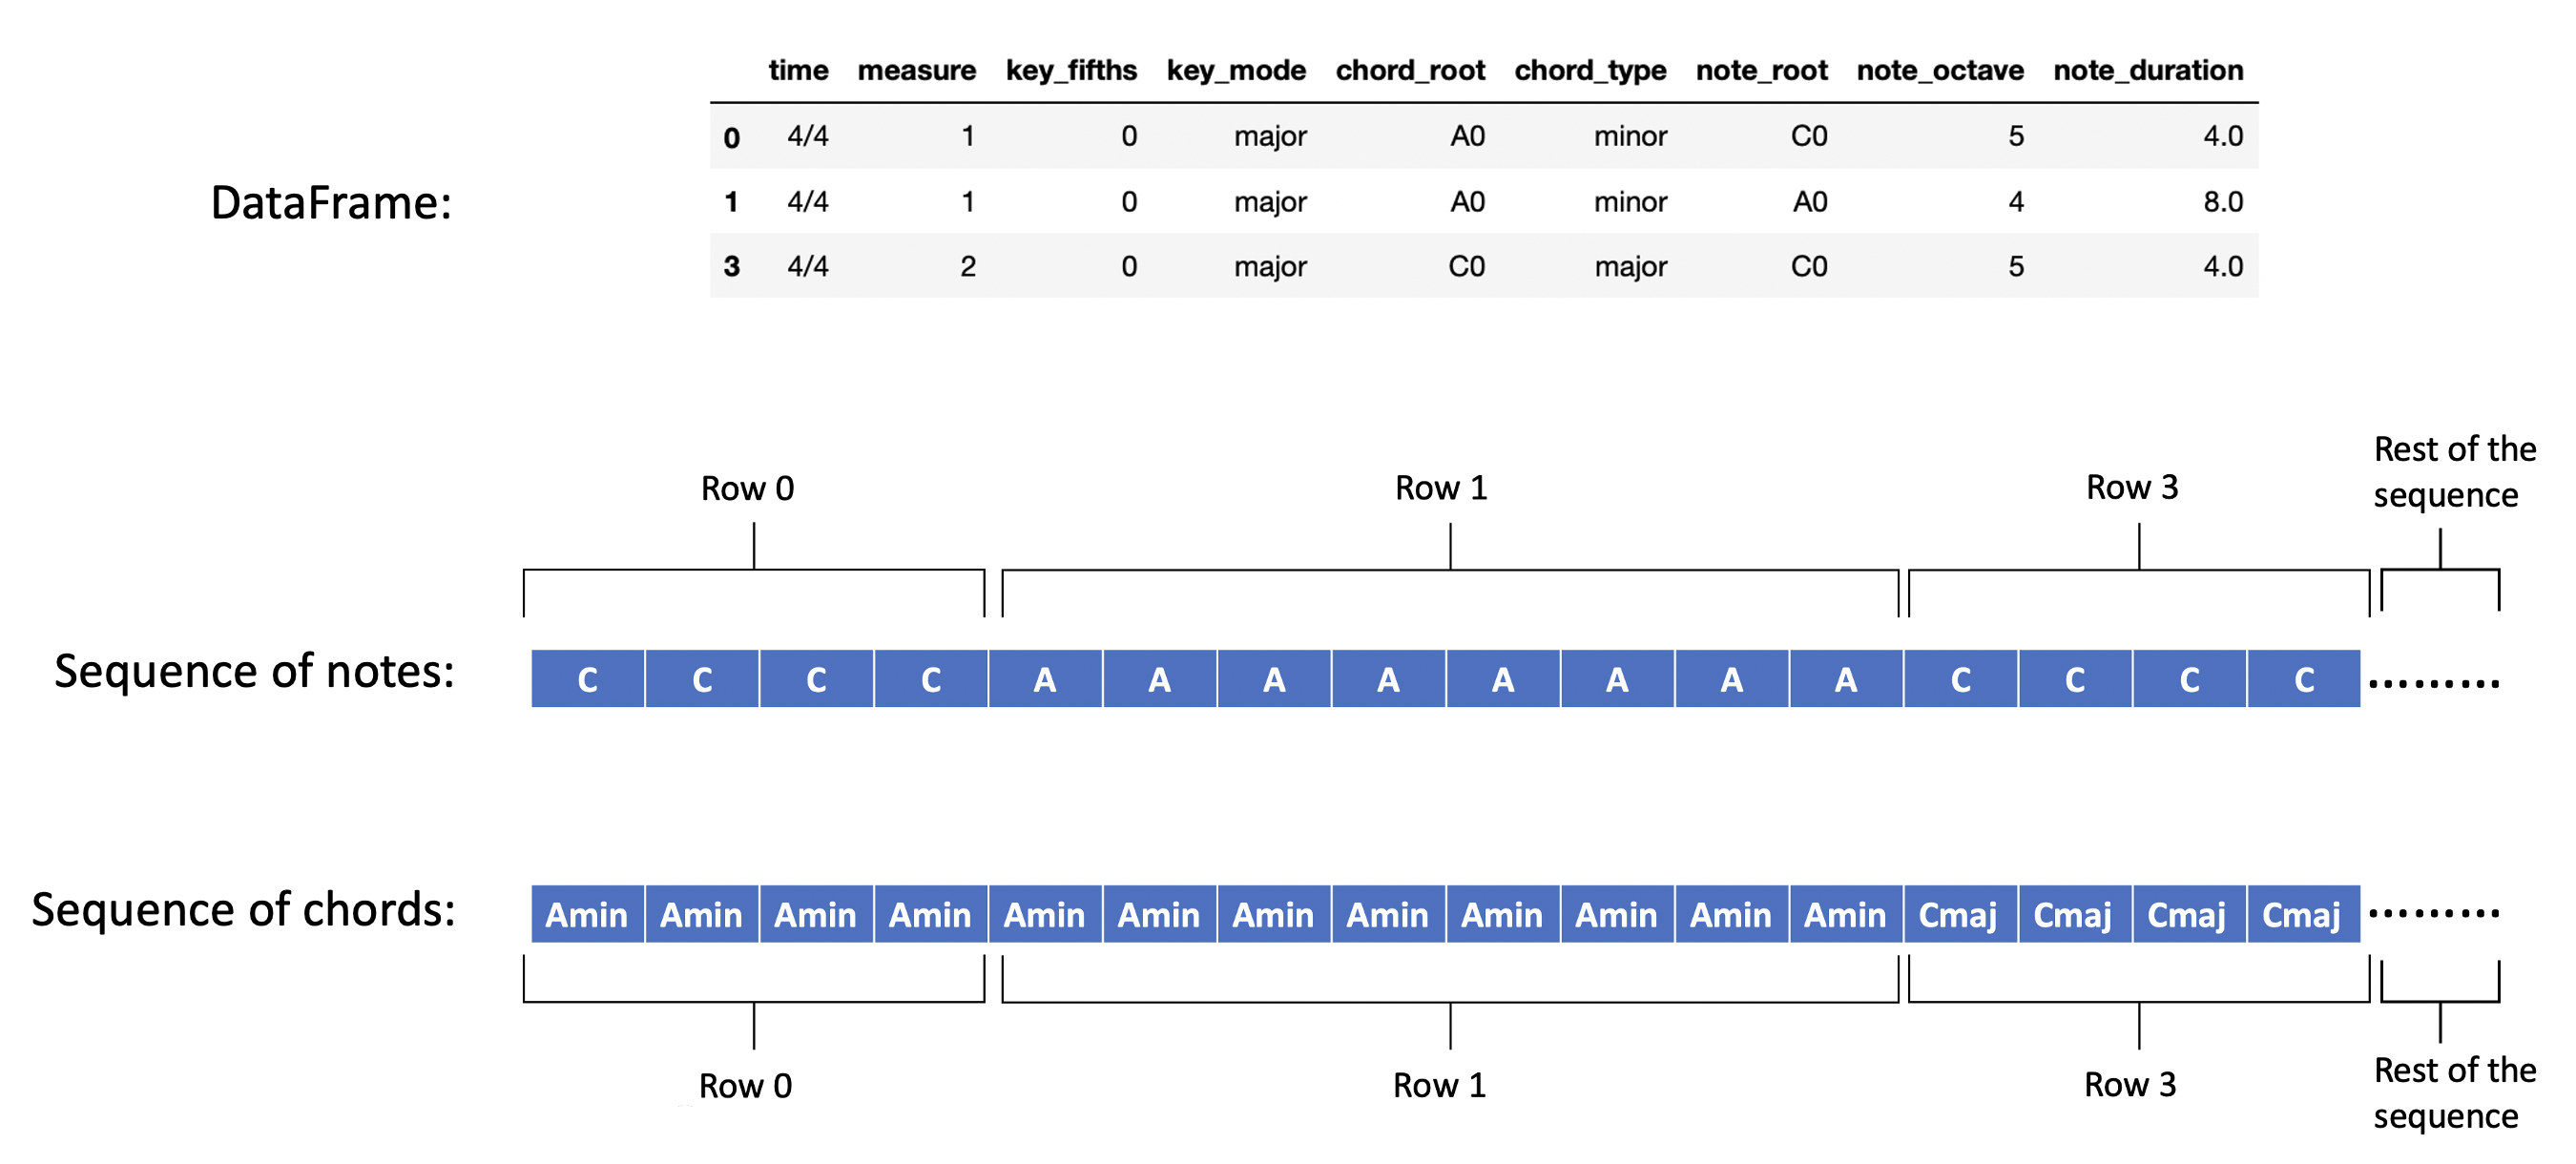
\includegraphics[width=0.4\columnwidth]{Figures/Transformer}
    \decoRule
    \caption{The architecture of a transformer from \cite{Transformers}}
    \label{fig:Transformer}
\end{figure}

\section{Our Model}

We propose the use of a conditional BLSTM GAN to learn the association between melodies and chords.
The Discriminator consists of a number of LSTM layers followed by a linear output layer.
The Generator consists of a linear layer followed by a number of LSTM layers and then by another linear layer.
The Binary Cross Entropy loss is used to determine the Discriminator loss for each example. This is averaged across every measure and then between real and generated examples
\subsection{Model Functionality}

As proof of concept for the design we developed a command line based interface for the model such that it was easy to train, vary parameters and test. 
In production the user would be able utilise a subset of this interface, such as the option to generate accompaniment and have it played back, through a graphical user interface.
The options available in the interface are show in table \ref{tab:parameters}

\begin{table}
    \caption{The parameters of the command line iterface for the model}
    \label{tab:parameters}
    \centering
    \begin{tabular}{l l l p{0.5\linewidth}}
    \toprule
    \tabhead{Parameter} & \tabhead{Options} & \tabhead{Default} & \tabhead{Description} \\
    \midrule
    \code{-input\_size} & \code{[input\_size]} & $12$ & The size of the input vector to the discrimiator representing the melody  \\
    \code{-output\_size} & \code{[output\_size]} & $25$ & The size of the output vector representing the chord played in each measure \\
    \code{-h\_size} & \code{[h\_size]} & $128$ & The size of the hidden layers in the LSTM layers \\
    \code{-n\_layers} & \code{[n\_layers]} & $2$ & The number of LSTM layers in the generator and discriminator \\
    \code{-noise\_size} & \code{[noise\_size]} & $12$ & The size of the noise vector concatinated with the input vector to the generator \\
    \code{-max\_seqlen} & \code{[max\_seqlen]} & $200$ & The maximum length of song in measures used in training \\
    \code{-src\_data} & \code{[src\_data]} &  & The default path to the training data \\
    \code{-batch\_size} & \code{[batch\_size]} & $10$ & The size of the batches used in the stochasitc gradient descent algorithm \\
    \code{-epochs} & \code{[epochs]} & $100$ & The number of epochs used in training \\
    \code{-printevery} & \code{[printevery]} & $10$ & The number of epochs between printing an example during training \\
    \code{-load} & & False & Whether to load a model in or not \\
    \code{-load\_dir} & \code{[load\_dir]} &  & The path to the folder containing pretrained models \\
    \code{-model\_num} & \code{[model\_num]} & $1$ & The number of the model to be loaded in \\
    \code{-save} & & False & Whether to save the model after training \\
    \code{-save\_dir} & \code{[save\_dir]} &  & The path to the save directory \\
    \code{-playback} & & False & Whether to play an example of generated music at the end of training \\
    \bottomrule \\
\end{tabular}
\end{table}
 

\section{Training}

\paragraph{Optimiser}
We used the Adam optimiser \cite{Adam} which is recommended in the Stanford \href{https://cs231n.github.io/}{CS231n: Convolutional Neural Networks for Visual Recognition}\footnote{https://cs231n.github.io/} as the default optimiser.
\textbf{EXPLAIN ADAM WHEN NOT FALLING ASLEEP}

\paragraph{Loss}
As we are using a GAN we use the Binary Cross Entropy or BCE as our loss function

\begin{equation}
\frac{1}{N} \sum_{i=1}^N log(p(y_i))
\end{equation}
which for the disciminator takes the form
\begin{equation}
    \frac{1}{N} \sum_{i=1}^N log(D(conc(x_i,z_i))) + log(1-D(conc(G(z_i),z_i)))
\end{equation}
where $x_i$ is are the real examples, $z_i$ are the melodies and the $conc$ function concatinates the two vector arguments.
The loss is the sum of the loss of the discriminator on real data and generated data.
The generator loss is
\begin{equation}
    -\frac{1}{N} \sum_{i=1}^N log(1-D(conc(G(z_i),z_i)))
\end{equation}
which results in tring to maximise the loss of the discriminator on generated data.
This is equivalent to finding the discriminator loss on generated data when labeled as real which is the method we use in our implementation.

\subsection{Avoiding Overfitting}
Dropout
GAN techniques
Reducing number of LSTM layers
\subsection{Issues}
Training is conducted in batches of a given size.
It is unlikely that the size of the dataset is divisble by the batch size so the final batch is likely to be shorter than the others.
This initially casued problems, however, we were able to set the dimensions of relevant objects, such as the input noise to the generator, to be relative to the current batch size rather than the usual batch size thus solving the problem.
Softmaxing of outputs of generator
Device managment

\subsection{Testing}
\section{Results}
